\section{EnsembleDashVis}
\label{sec:EnsembleDashVis}

This section presents the history and development behind our fully virtual collaboration between volunteer researchers from multiple UK institutions.
Being one of the four VIS volunteer teams, we received guidance from the RAMPVis team via regular virtual meetings. The RAMPVis team communicated with the SCRC modeling team regularly and provided us with important information and data.
We chronicle the development of different views of the data, the order in which they were introduced, and the reasons and motivations at the time.
In 2020 we were all in an unprecedented and unfamiliar situation, thus, some of our decisions were ad-hoc.

Please refer to the Supplementary Materials for high-resolution figures of all five views detailed in this section.

\bobgraph{Meeting \#1 - July 2020}

\label{subsec:InitialMeeting}
On 27 July 2020, amid the UK's first national lockdown and stricter measures imposed by local authorities, we convened the initial virtual meeting with VIS researchers from King's College London, Loughborough University, Swansea University, University of Nottingham, University of Warwick, and University of Oxford.

During the meeting, we received an overview of the SCRC and the responsibilities of the visualization volunteer team.
Our assigned task was to create visual interfaces for the model, for the purpose of enabling the modelers to analyze the outcomes of the model.

Following the initial meeting, we engaged in email correspondence with the modelers to delve into the visualization requirements. The modelers shared a comprehensive list of parameters and model outcomes, along with the corresponding outcome data \cite{scrc2020Covid19}.

\bobgraph{Commit \#1 - Sep 2020}

We proceeded to create an initial prototype of the visualization, which was subsequently reviewed by the modelers.
Incorporating their input, we refined the prototype during our weekly internal discussions.
On 14 Sep 2020, England introduced the `rule of six', which banned any gatherings above six.
On the same day, we made our first commit to a GitHub repository, signifying the commencement of our development\footnote{\url{https://github.com/thevisgroup/EnsembleVis}}.
At the same time, we began preprocessing the data.
A week after the initial commit, the UK witnessed the implementation of additional restrictions, such as mandatory work from home and a 10PM curfew.

\bobgraph{Meeting \#2, View \#1 - Nov 2020}

On 5 Nov 2020, the first day of the second national lockdown in the UK, we completed the first view of the simulated input parameters, a parallel coordinates plot.
See \Cref{fig:pc1}.
We chose to use a parallel coordinates plot as it is a common technique for visualizing multivariate data, and is particularly useful to explore relationships and patterns across multiple input parameters.
Each axis in the plot represents an input parameter, the y-axis represents the value of the parameter, and each polyline represents one input configuration. 
The plot supports brushing and linking, enabling modelers to select a subset of input parameters to focus on interesting configurations.
This followed by the second meeting with the RAMPVis team from other institutions, where we received feedback on the first view, on 6 Nov 2020.
% Revision
The response from the modelers to the parallel coordinates view was, in general, very positive.  
They are very interested in multivariate analysis and had not seen this visual representation before.  
More details are provided in Section~\ref{sec:feedback} on domain expert feedback.

\begin{figure}[tb!]
    \centering
    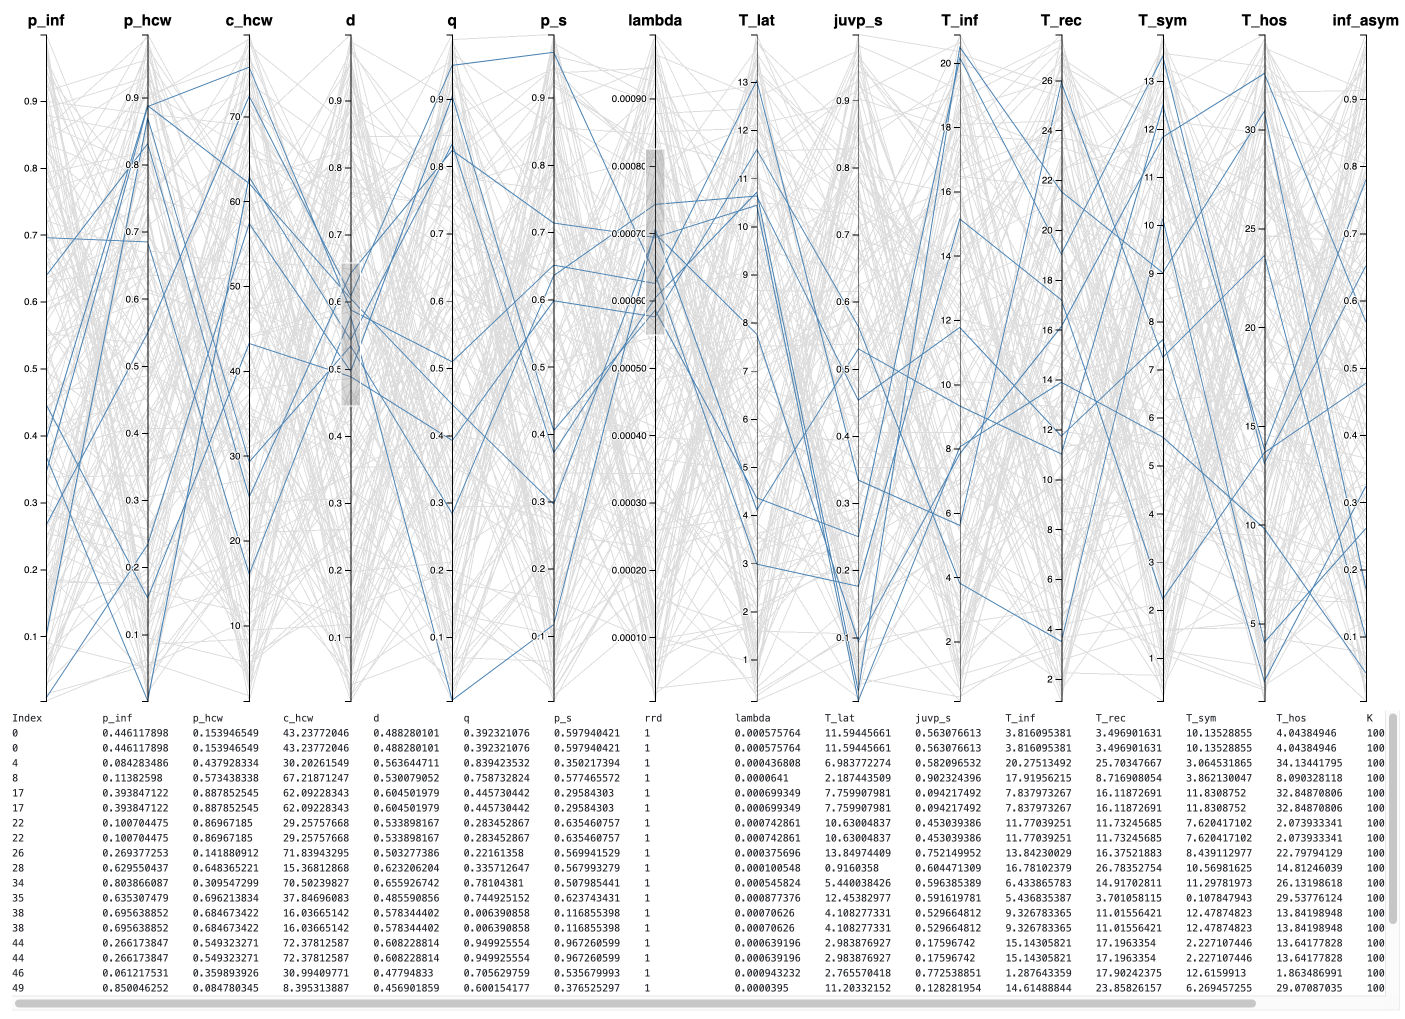
\includegraphics[width=\linewidth]{pc1.png}
    \caption{The first visual design, a parallel coordinates plot depicting all 160 input configurations of the model, was completed on 5 Nov 2020. 
    Each axis represents an input parameter, the y-axis represents the value of the parameter, and each polyline represents one input configuration.
    The table below shows the configuration details.
    }
    \label{fig:pc1}

\end{figure}

\bobgraph{Meeting \#3, View \#2 - Nov 2020}

On 11 Nov 2020, the group convened for the third meeting, where we received further feedback from the RAMPVis team on the parallel coordinates plot. As per the modelers' requests conveyed via email, we incorporated a line chart to depict the model outcomes.
See \Cref{fig:1st-line}.
The x-axis of the chart corresponds to the number of days since the first date in the Scottish dataset, while the y-axis represents the population.
Line chart and other classic visual designs are widely used by the modelers, they are familiar with these designs and can easily interpret the results.
The line chart is coordinated with the parallel coordinates plot, enabling the modelers to select a subset of the input parameters and quickly identify the corresponding model outcomes.
A focus+context technique is used to highlight the selected subset of the input parameters in the parallel coordinates plot.

\begin{figure}[tb!]
    \centering
    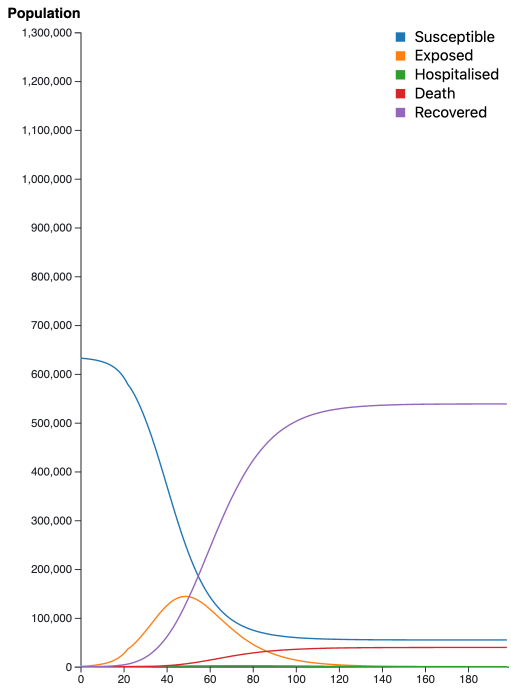
\includegraphics[width=\linewidth]{1st-line.png}
    \caption{A line chart depicting the model outcomes.
    The x-axis of the chart corresponds to the number of days since the first date in the Scottish dataset, while the y-axis represents the population.
    To differentiate between different population categories, a color map was incorporated: \textcolor{DodgerBlue1}{susceptible}, \textcolor{Chocolate1}{exposed}, \textcolor{Green4}{hospitalized}, \textcolor{red}{recovered}, \textcolor{DarkOrchid1}{death}, \textcolor{LightSalmon4}{asymptomatic}, and \textcolor{HotPink1}{symptomatic}.
    The focus+context technique is used here to highlight the outcome of the current configuration, while the grey lines represent other outcomes. On day 20, there is an unusual spike which was later identified as caused by an error in the model.
    }
    \label{fig:1st-line}

\end{figure}

\bobgraph{Meeting \#4, View \#3 - Nov 2020}

On 25 Nov 2020, the group convened for the fourth meeting, held just a day after the announcement of the gathering rules for Christmas in the UK.
During the meeting, we received feedback from the RAMPVis team on the new view of the input parameters, a table with glyphs.
See \Cref{fig:table-view}.
We incorporated this table view featuring glyphs to depict all 160 input parameter configurations, following discussions with the modelers.
Each row represents an input configuration, and each column represents an input parameter.
The table view enables the modelers to sort configurations by individual input parameters.
Each parameter value is symbolized by a bar glyph, the color and length correspond to its deviation from the average value of 160 predictions.

The table view provides the functionality to sort the parameters according to their values and can be dynamically updated by brushing the parallel coordinates plot for the input parameters in \Cref{fig:pc1}.
The line chart in \Cref{fig:1st-line} can be quickly updated to display the corresponding model outcomes by clicking on the configuration index in the table view.

\begin{figure}[tb!]
    \centering
    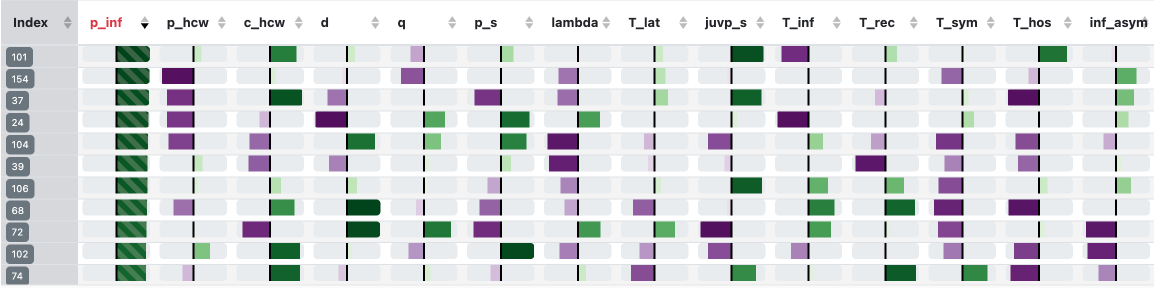
\includegraphics[width=\linewidth]{table.png}
    \caption{The table view depicting all 160 input parameter configurations.
    The view enables the modelers to sort parameter values and identify interesting configurations.
    Each row represents an input configuration, and each column represents an input parameter.
    Upon clicking on a row, the line chart in \Cref{fig:1st-line} is updated to display the corresponding model outcomes.
    Clicking on the column header sorts the table by the parameter values.
    }
    \label{fig:table-view}

\end{figure}

\bobgraph{Meeting \#5 - Dec 2020}

On 9 Dec 2020, a week after the end of the second national lockdown in the UK, with England facing a stricter three-tier restriction policy, the group convened for the fifth meeting.
At this point, we still had not met with the modelers, all communications and discussions took place via email.
The RAMPVis team decided to organize a meeting with the modelers to present our prototype for feedback.

\bobgraph{Meeting \#6, Views \#4 \& 5, Feedback \#1 - Dec 2020}

On 10 Dec 2020, we finally met with modelers from Durham University, the University of Edinburgh, the University of Exeter, the University of Glasgow, the London School of Hygiene \& Tropical Medicine, for the first time.
In contrast to sharing screenshots via email and deploying a website with a live view of our development (which they might not have been proficient in using), we delivered a live presentation, fielding numerous questions.
The modelers were pleased with the dashboard, and a list of ad-hoc requirements was provided. Furthermore, we collected insightful feedback that we elaborate on in detail in \Cref{sec:feedback}.
\begingroup
\begin{enumerate}[itemsep=0pt,topsep=0pt]
    \item The modelers found that the parallel coordinates plot is useful in identifying outliers, and requested the incorporation of another one for the model outcomes.
    Given that the outcome data mirrors the input in a multivariate format, employing a parallel coordinates plot could potentially be useful.
    We implemented this as shown in \Cref{fig:pc2}.
    \item The modelers requested that all the simulation results be displayed in the line chart, with the current one highlighted.
    This resembles their usual workflow for analyzing multiple simulation outcomes.
    We implemented this as shown in \Cref{fig:1st-line}.
    \item The modelers requested the incorporation of a scatterplot to visualize the model outcomes, specifically a Principal Component Analysis (PCA) result obtained from another VIS volunteer team.
    The motivation behind this is to reduce the dimensionality and identify key parameters.
    We implemented this as shown in \Cref{fig:pca}.
    \item The modelers requested all views to be coordinated with each other, enabling observation of relationships between input parameters and model outcomes through interaction. 
    \begin{enumerate}[itemsep=0pt,topsep=0pt]
        \item Brushing on the input parallel coordinates plot (\Cref{fig:pc1}) highlights the corresponding input configurations in both the table view (\Cref{fig:table-view}) and scatterplot (\Cref{fig:pca}).
        \item Brushing on the scatterplot (\Cref{fig:pca}) for input configurations highlights the corresponding input configurations in both the table view (\Cref{fig:table-view}) and input parallel coordinates plot (\Cref{fig:pc1}).
        \item Clicking on a specific row in the table view (\Cref{fig:table-view}) renders the corresponding output data in both the output parallel coordinates plot (\Cref{fig:pc2}) and line chart (\Cref{fig:1st-line}).
    \end{enumerate}
\end{enumerate}
\endgroup

Furthermore, we received the exciting news that initial funding had been successfully secured \cite{engineering&physicalsciencesresearchcouncil2021RAMP}, which led to the transition of our volunteer work to a team of paid developers, who would continue with further implementation of the project.

\begin{figure}[tb!]
    \centering
    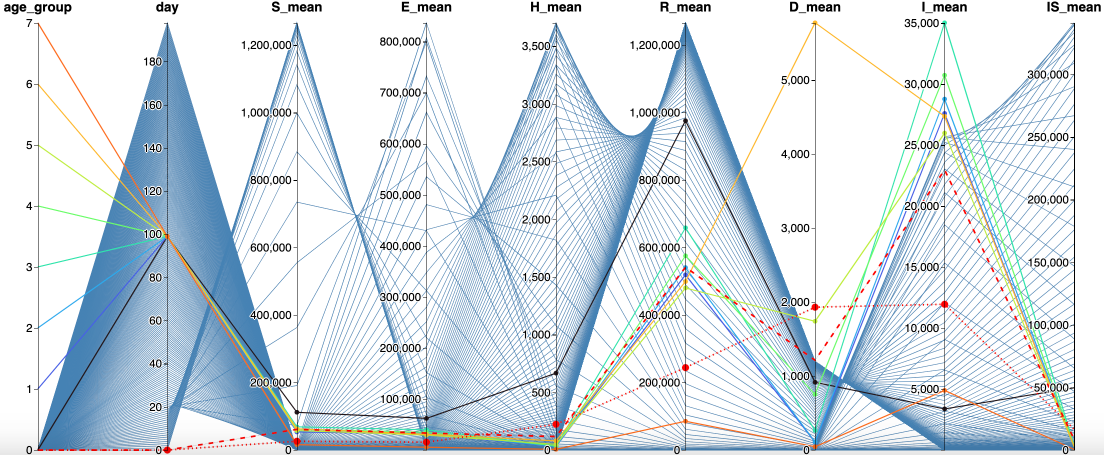
\includegraphics[width=\linewidth]{pc2.png}
    \caption{A parallel coordinates plot depicting the model outcomes by age group. As requested by the modelers, the mean value of 160 predictions generated by each input configuration, as well as for each age group, was computed and rendered here. Each axis represents one variable from the outcome and \textcolor{SteelBlue4}{its value}.
    Each age group is mapped to a color, the dashed red line {\textcolor{red}{\rule[0.2ex]{0.1cm}{0.5pt}\hspace{0.1cm}\rule[0.2ex]{0.1cm}{0.5pt}\hspace{0.1cm}\rule[0.2ex]{0.1cm}{0.5pt}\hspace{0.1cm}}}
    represents the average value, and the dotted red line \textcolor{red}{\dotfill} represents the standard deviation.
    }
    \label{fig:pc2}

\end{figure}

\begin{figure}[tb!]
    \centering
    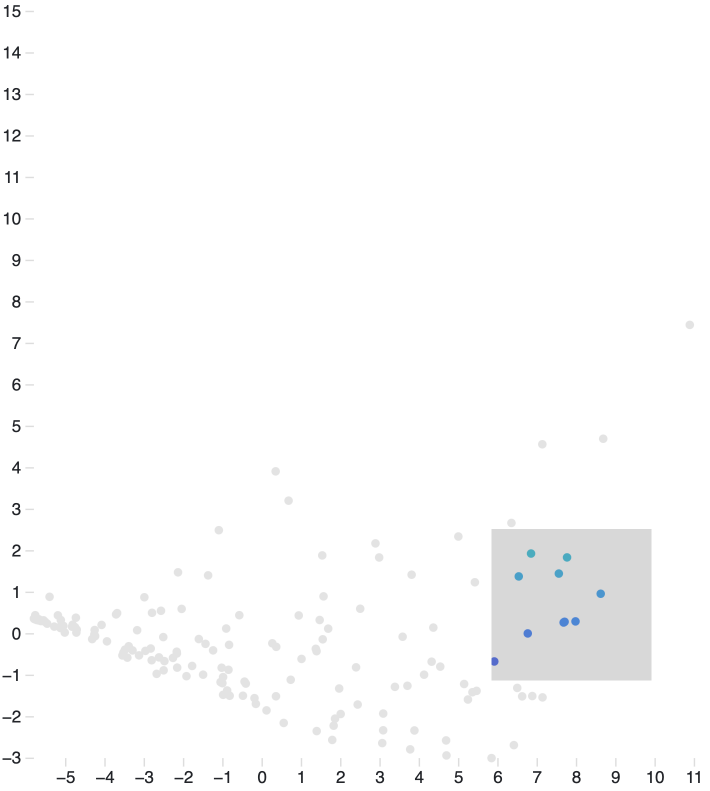
\includegraphics[width=0.6\linewidth]{pca.png}
    \caption{A scatterplot depicting the PCA outcome from another VIS volunteer group, was added upon request by the modelers. Upon brushing, the selected configurations are highlighted in the table view in \Cref{fig:table-view}.
    }
    \label{fig:pca}

\end{figure}

\bobgraph{Meeting \#7, Feedback \#2 - Mar 2021}
On 25 Mar 2021, the UK was in the process of cautiously lifting its third national lockdown, the `rule of two' was still in place.
The group convened for the seventh meeting, where we received further feedback from the modeling team on our implementation.
We detail the feedback in \Cref{sec:feedback}.

\bobgraph{Last Commit - Apr 2021}

By 28 Apr 2021, more restrictive measures were abolished, although the prohibition on mixing between households was still in effect.
On this day, we made our last commit to our GitHub repository. This act signified the completion of our volunteer work, as we had smoothly transitioned all tasks to a team of paid developers.

During the entire development process, our meetings were exclusively conducted virtually, and our communication relied heavily on email correspondence.
Despite the lack of in-person interactions, we successfully met the initial requirements of the modelers and delivered a \ac{VIS} solution that received very positive feedback from the SCRC modeling team.

\bobgraph{Meeting \#8, Feedback \#3 - May 2021}
On 19 May 2021, the UK was viewing the light at the end of the Covid tunnel, weddings and funerals were still restricted to 30 people, and indoor gatherings of more than two households were still banned.
The group convened for the eighth and final volunteer meeting.
During this final meeting, a modeler joined and gave us some in-depth feedback on the influence our work had on their modeling process, as well as suggesting potential improvements.
We detail the feedback in \Cref{sec:feedback}.
